% $Id: preadjustment.tex 5860 2018-01-23 22:23:18Z mskala $

%
% MSK 007 pre-adjustment procedure
% Copyright (C) 2017  Matthew Skala
%
% This program is free software: you can redistribute it and/or modify
% it under the terms of the GNU General Public License as published by
% the Free Software Foundation, version 3.
%
% This program is distributed in the hope that it will be useful,
% but WITHOUT ANY WARRANTY; without even the implied warranty of
% MERCHANTABILITY or FITNESS FOR A PARTICULAR PURPOSE.  See the
% GNU General Public License for more details.
%
% You should have received a copy of the GNU General Public License
% along with this program.  If not, see <http://www.gnu.org/licenses/>.
%
% Matthew Skala
% https://northcoastsynthesis.com/
% mskala@northcoastsynthesis.com
%

\chapter{Pre-adjustment}\label{ch:preadj}

To complete the preadjustment process you will need an
ohmmeter; a tool (probably a small slotted screwdriver) to adjust the
trimmers; and your completed Board~3.  A Eurorack power supply and voltmeter
are optional.

Note this procedure is to be done on
Board~3 \emph{disconnected} from any other boards; the measurements will not
be correct if it is attached to the other boards. 
Figure~\ref{fig:board3-silk} shows the silkscreen art for Board~3, which may
help to locate the trimmers and test points.  Version~3 of the art is
shown; if you have one of the earlier Version~2 boards, all the trimmers and
test points are in the same places, but there are minor differences in some
of the label positions.

Throughout these instructions, calculated target values for the measurements
are given to more precision than it is usually practical to measure or
adjust.  Just round them off to the appropriate level for what your test
equipment can do.

\begin{figure*}
\centering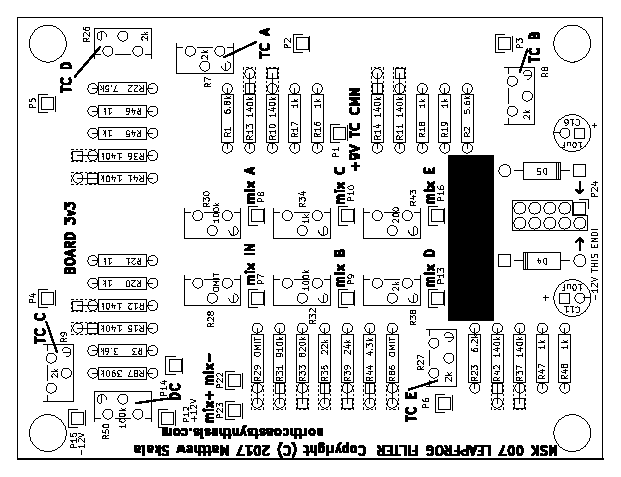
\includegraphics[angle=-90,scale=1.5]{board3-silk.eps}
\caption{Board~3 silkscreen art}\label{fig:board3-silk}
\end{figure*}

\section{Short-circuit test}

This check will be done again on the entire module during the regular
adjustment phase, but it's worth doing it right at the start on Board~3
alone to help narrow down any problems you might discover.

The two pins on the Eurorack power connector nearest the edge of Board~3
(at the bottom when the module is mounted upright in a case) are for the
$-$12V connection.  That is the end where the red stripe on the cable would
normally connect.  The two pins at the other end of the connector (furthest
from the edge of the board) are for $+$12V power.  All six pins in the
middle are for 0V (ground).

\noindent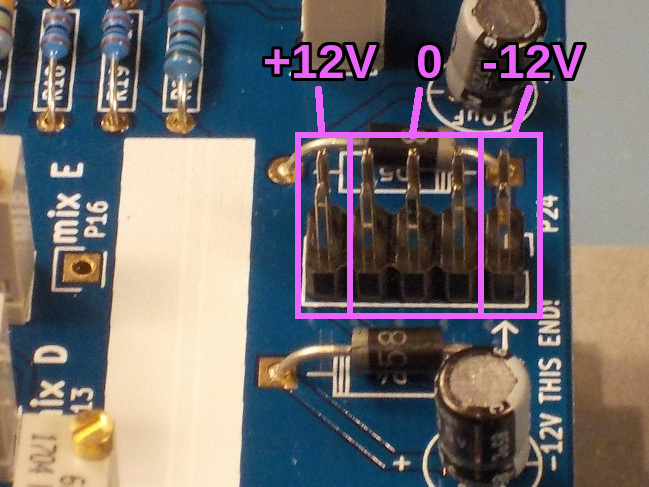
\includegraphics[width=\linewidth]{power-pinout.jpg}

Check for shorts between the three power connections, testing each pair in
both directions (six tests in all).  Ideally, you should use an ohmmeter's
``diode test'' range for this, and it should read infinite in the reverse
direction (positive lead to $-$12V and negative lead to each of the other
two, as well as positive lead to ground and negative to $+$12V) and greater
than 1V in the forward direction (reverse those three tests).  If any of
these six measurements is less than 100$\Omega$ or 1V, then something is
wrong with the build and you should troubleshoot it before applying power.

\section{Integrator time constants}

Each of the five integrator stages has a time constant controlled primarily
by a trimmer.  At this point we set these roughly by setting the resistances
to values that would be correct if all other components in the circuit had
their design values; in the later, more precise adjustment step, the values
may be modified to compensate for variations in those other components.

Measure the resistance between P1 ``+9V TC CMN'' (that is, ``time constant
common''; the test point is connected to what will be the internal +9V
supply when the module is fully assembled) and P2 ``TC~A'' and adjust R7 to
bring this resistance to 7.9856k$\Omega$.

Measure the resistance between P1 ``+9V TC CMN'' and P3 ``TC~B'' and adjust
R8 to bring this resistance to 6.8802k$\Omega$.

Measure the resistance between P1 ``+9V TC CMN'' and P4 ``TC~C'' and adjust
R9 to bring this resistance to 4.4816k$\Omega$.

Measure the resistance between P1 ``+9V TC CMN'' and P5 ``TC~D'' and adjust
R26 to bring this resistance to 8.1997k$\Omega$.

Measure the resistance between P1 ``+9V TC CMN'' and P6 ``TC~E'' and adjust
R27 to bring this resistance to 7.4310k$\Omega$.

\section{Output mix}

The output of the filter is a carefully chosen fixed mixture of the output
signals from the five integrator stages.  There is an interaction between
the R43 and R34 adjustments, hence their repetition in these instructions;
the stated sequence should minimize any problems caused by interaction.

Measure the resistance between P22 ``mix~$-$'' and P16 ``mix~E'' and adjust
R43 to bring this resistance to 4.2802k$\Omega$.

Measure the resistance between P23 ``mix~$+$'' and P13 ``mix~D'' and adjust
R38 to bring this resistance to 25.144k$\Omega$.

Measure the resistance between P22 ``mix~$-$'' and P10 ``mix~C'' and adjust
R34 to bring this resistance to 19.3130k$\Omega$.

Measure the resistance between P23 ``mix~$+$'' and P9 ``mix~B'' and adjust
R32 to bring this resistance to 890.04k$\Omega$.

Measure the resistance between P22 ``mix~$-$'' and P8 ``mix~A'' and adjust
R30 to bring this resistance to 961.04k$\Omega$.

Measure the resistance between P22 ``mix~$-$'' and P16 ``mix~E'' a second
time; it should be near 4.2802k$\Omega$.  If necessary, adjust
R43 to make it exactly 4.2802k$\Omega$.

Measure the resistance between P22 ``mix~$-$'' and P10 ``mix~C'' a second
time; it should be near 19.3130k$\Omega$.  If necessary, adjust
R34 to make it exactly 19.3130k$\Omega$.

Note the footprint labelled R28, corresponding to the test point P7
``mix~IN,'' is meant for reusing this board design with other filter curves;
in the standard lowpass configuration there is no trimmer there and no
adjustment needed.

\section{DC offset trim}

The DC offset trimmer R50 should be set to its midpoint for now; it
will be adjusted up or down to compensate offset in the OTA chips later.
If you followed the build instructions carefully, then you will have set it
to its midpoint before installing it and no further adjustment is needed at
this point.

Otherwise, connect the board to a Eurorack power supply, and confirm that
+12V appears on test point P12 and -12V on P15, relative to any convenient
grounded point on the board (such as the mounting hole nearby) and to within
the voltage tolerance of your power supply.  Measure the voltage on P14
labelled ``DC'' and adjust R50 to bring the measured voltage to zero.

Alternate procedure:  instead of connecting the board to a power supply, you
can measure the resistances among P14, P12 (labelled $+$12V), and P15
(labelled $-$12V).  The wiper of the 100k$\Omega$ trimmer is connected to
P14 and the two ends of the track are connected to P12 and P15, so with no
power applied to the board, you can adjust for equal resistances (of
50k$\Omega$ subject to tolerance) between P12 and P14 and between P14 and
P15.
